\documentclass[t, 11pt,xcolor=dvipsnames, aspectratio=169]{beamer}

% Insert number of slides defining a common footline for all slides
\beamertemplatenavigationsymbolsempty
\setbeamertemplate{footline} { \hspace{0.1cm} 
\includegraphics[scale = 0.03]{logos/chaos_logo_black_without_bkg.png} \hspace*{13cm}{\small \insertframenumber/\inserttotalframenumber}\vspace{3pt}} 

% Define colors useful for presentation
\definecolor{maincolor}{RGB}{0,102,204}
\definecolor{hcolor}{RGB}{255,128,0}
\definecolor{mygreen}{RGB}{120,190,33}

% Set colors for the presentation and references
\setbeamercolor{title}{fg=maincolor}
\setbeamercolor{frametitle}{fg=maincolor}
\setbeamercolor{structure}{fg=maincolor}
\setbeamercolor{footline}{fg=black}
\setbeamercolor{caption name}{fg=black}
\setbeamercolor{bibliography item}{fg=black}
\setbeamercolor*{bibliography entry title}{fg=black}
\setbeamercolor*{bibliography entry author}{fg=black}
\setbeamercolor*{bibliography entry location}{fg=black}
\setbeamercolor*{bibliography entry note}{fg=black}

\setbeamertemplate{section in toc}[sections numbered]
\setbeamertemplate{caption}[numbered]
\setbeamertemplate{bibliography item}{\insertbiblabel}
\usepackage[font=small,labelfont=bf]{caption}

%Additional packages
\usepackage{amsmath}
\usepackage{amsfonts}
\usepackage{amssymb}
\usepackage{appendixnumberbeamer}
\usepackage{pbox}
\usepackage{multirow}
\usepackage[makeroom]{cancel}
\usepackage[export]{adjustbox}
\usepackage{siunitx}
\usepackage{subcaption}
\usepackage{wrapfig} %To wrap figures

% Framed and shaded text: useful to hcolor information
\usepackage{framed, color}
\definecolor{shadecolor}{RGB}{220,220,220}

% Tikz packages for diagrams
\usepackage{tikz}
\usetikzlibrary{arrows,shapes,positioning,shadows,trees, calc, chains}

% Useful acronyms for some math functions
\newcommand{\dd}{\mathrm{d}} % differential d
\newcommand{\pp}[1]{\left( #1 \right)} % easy way to do parenthesis

% Deal.ii font
\newcommand{\dealii}[1]{{\fontfamily{qcr}\selectfont #1}}

% Change the label of the figure
\renewcommand{\figurename}{Fig.}


%-------------------------
% Title page
%-------------------------
% Details for title page
% Commenting the line below will make the title page centered
\setbeamertemplate{title page}[default][left,colsep=-4bp,rounded=true,shadow=\beamer@themerounded@shadow]

% Title of the presentation
\title{\textbf{Title of the presentation}}

% Subtitle of the presentation
\subtitle{Subtitle}

% List of authors. Good idea to put your name in bold if you are not the first author
\author{Mama Bear, \textbf{Papa Bear}, Child Bear \\ CHAOS laboratory \\ Department of Chemical Engineering \\ Polytechnique Montréal}

% Logo of the laboratory and the university
\titlegraphic{
\includegraphics[width=4.2cm]{logos/chaos_logo_black_without_bkg.png}\hspace*{6.8cm}~%
   
\includegraphics[width=3cm]{logos/Polytechnique_signature-RGB-droite_ENG.png}
}

% Add an outline slide at the beginning of each new section
\AtBeginSection[]
{
  {
  \setbeamertemplate{footline}{} %this line removes slides numbers
  \begin{frame}[noframenumbering]
    \frametitle{Table of Contents}
    \tableofcontents[currentsection]
  \end{frame}
  }
}


\begin{document}
% Title slide
{
\setbeamertemplate{footline}{} %this line removes slide number
\begin{frame}[noframenumbering]
  \titlepage
\end{frame}
}
	
% Contents slide
{
\setbeamertemplate{footline}{} %this line removes slide number
\begin{frame}[noframenumbering]
  \frametitle{\textbf{Outline}}
  \tableofcontents
\end{frame}
}
	
% Other slides
\section{Motivation}
\begin{frame}{Slide}
    This is a regular slide with only text.             These are kinda boring.
\end{frame}




\begin{frame}{Slide with grey box and columns}
	\visible<1->
	{\begin{shaded}
			\textbf{Lethe} leverages high-order continuous Galerkin FEM to simulate multiphase flow in chemical engineering applications (reactors, mixers, etc.)
	\end{shaded}}
	
	\begin{minipage}[t]{0.48\linewidth}
		%\visible<2->
		{
			\begin{block}{Solid open-source foundation}
				\begin{itemize}
					\item Based on the deal.II framework
					\item \textbf{Tested}: $>330$ tests
					\item \textbf{Documented}: $>50$ examples
					\item Used in 6 countries (Canada, Germany, UK, Australia, China, USA)
				\end{itemize}
			\end{block}
		}
	\end{minipage}%
	\hfill%
	%
	\begin{minipage}[t]{0.48\linewidth}
		%\visible<3->
		{
			\begin{block}{Applications}
				\begin{itemize}
					\item Fluidized and spouted-bed reactors
					\item Laser powder bed fusion
					\item Free surface flows in containers
					\item DNS of particle-laden flow
					\item Mixing in stirred tanks 
					\item Flow in porous media
				\end{itemize}
			\end{block}
		}
	\end{minipage}
\end{frame}



\begin{frame}
	\frametitle{\textbf{Problem: Navier-Stokes equations}}
	
	Consider a $d$-dimensional domain $\Omega$ and the following problem subjected to homogeneous Dirichlet boundary conditions: 
	%\vspace{0.1cm}
	\begin{columns}[c]
		\begin{column}{0.5\textwidth}
			% \vspace*{-\baselineskip}
			\begin{framed}
				Find a vector $\vec{u}$ and a scalar $p$ in $\Omega \rightarrow \mathbb{R}$ satisfying:
				\begin{align*}
					\nabla \cdot \vec{u} &= 0 \\
					\partial_{t} \vec{u} + (\vec{u} \cdot \nabla) \vec{u} + \nabla p - \nu \Delta \vec{u} - \vec{f} &= 0
					% \vec{u} &= 0 \ \textrm{ in } \partial\Omega
					% \textrm{ in } \Omega
				\end{align*}
			\end{framed}
		\end{column}
		\begin{column}{0.4\textwidth}
			\vspace*{-\baselineskip}
			\begin{center}
				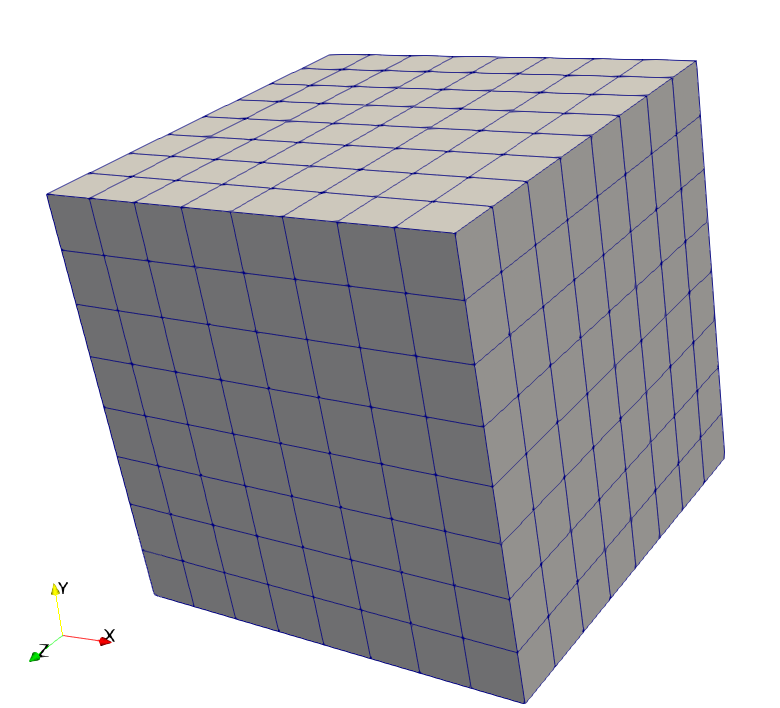
\includegraphics[scale = 0.13]{images/domain_3d.png}
			\end{center}
		\end{column}
	\end{columns}
	
	\vspace{0.4cm}
	\begin{itemize}
		\item This is a coupled problem for velocity ($\vec{u}$) and pressure ($p$).
		\item This is a non-linear problem due to the second term in the momentum equation.
	\end{itemize}    
\end{frame}
	


\begin{frame}
	\frametitle{\textbf{Problem: Variational formulation}}
	%\fontsize{10.5}{11}\selectfont
	We multiply by the test functions $\vec{v}$ and $q$, and integrate over the domain using the notation $(a, b)_{\Omega} = \int a b \ \text{d}\Omega$:
	\begin{align*}
		\left( q, \nabla \cdot \vec{u} \right)_{\Omega} + (\vec{v}, \partial_t \vec{u} + (\vec{u} \cdot \nabla) \vec{u} + \underbrace{\nabla p}_{1} - \underbrace{\nu \Delta \vec{u}}_{2} - \vec{f} )_{\Omega} = 0
	\end{align*}
	We integrate by parts terms $1$ and $2$:
	\begin{align*}
		(\vec{v}, \nabla p)_{\Omega} = - (\nabla \cdot \vec{v}, p)_{\Omega} + ( \vec{n} \cdot \vec{v}, p)_{\partial\Omega} \\
		(\vec{v}, -\nu \Delta \vec{u})_{\Omega} = \nu (\nabla \vec{v}, \nabla \vec{u})_{\Omega} - (\vec{v} \vec{n}, \nu \nabla \vec{u})_{\partial\Omega} 
	\end{align*}
	If we assume Dirichlet B.Cs or zero stress conditions on $\partial\Omega$:
	\begin{align*}
		( \vec{n} \cdot \vec{v}, p)_{\partial\Omega} - (\vec{v} \vec{n}, \nu \nabla \vec{u})_{\partial\Omega} = 0
	\end{align*}
	%which is an outlet boundary condition where the normal stress is zero. Approximately empose an outlet boundary condition with a zero average pressure.
	Writing everything together we get the final weak form:
	\begin{align*}
		F(\vec{u}, p) := \left( q, \nabla \cdot \vec{u} \right)_{\Omega} + (\vec{v}, \partial_t \vec{u})  + \textcolor{maincolor}{(\vec{v}, (\vec{u} \cdot \nabla) \vec{u})_{\Omega}} \\
		- (\nabla \cdot \vec{v}, p)_{\Omega} + \nu (\nabla \vec{v}, \nabla \vec{u})_{\Omega} - (\vec{v}, \vec{f})_{\Omega}  = 0
	\end{align*}
	%\visible<2->{
	%	\textcolor{maincolor}{$\longrightarrow$ due to the non linearity we use \textbf{Newton's method} to solve this problem.}}
\end{frame}

\begin{frame}
	\frametitle{\textbf{Problem: SUPG/PSPG stabilization}}
	%\fontsize{10.5}{11}\selectfont
	Two stabilizing terms are added to the weak form $F$:
	\begin{align*}
		F &+ \underbrace{\sum_{k} {(\textcolor{red}{\tau} \nabla \cdot q, \partial_t \vec{u} + (\vec{u} \cdot \nabla) \vec{u} + \nabla p - \nu \Delta \vec{u} - \vec{f})}_{\Omega_k}}_{\text{\textcolor{mygreen}{PSPG term}}} \\
		&+ \underbrace{\sum_{k} {(\textcolor{red}{\tau}(\vec{u} \cdot \nabla) \vec{v}, \partial_t \vec{u} + (\vec{u} \cdot \nabla) \vec{u} + \nabla p - \nu \Delta \vec{u} - \vec{f})}_{\Omega_k}}_{\text{\textcolor{hcolor}{SUPG term}}}= 0
	\end{align*}
	where:
	\begin{align*}
		\textcolor{red}{\tau} = \left( \left( \frac{1}{\Delta t}\right)^2 + \left( \frac{2 \| \vec{u}\|}{h_{\text{conv}}} \right)^2 + 9 \left( \frac{4\nu}{h^2_{\text{diff}}} \right)^{2}\right)
	\end{align*}
	We take $h_{\text{conv}} = h_{\text{diff}} = h$, where $h$ is defined as follows:
	\begin{align*}
		h_{\text{2D}} = \sqrt{\frac{4 h_{k}}{\pi}} \ \ \ h_{\text{3D}} = \left( \frac{6 h_{k}}{\pi} \right)^{\frac{1}{3}}
	\end{align*}
%	
%	\visible<2->{
%		\textcolor{maincolor}{$\longrightarrow$ how is the \textbf{Jacobian} with the stabilization?}}
	
\end{frame}
	
\begin{frame}[noframenumbering, plain]
    \begin{tikzpicture}[remember picture, overlay]
        \node at (current page.center) {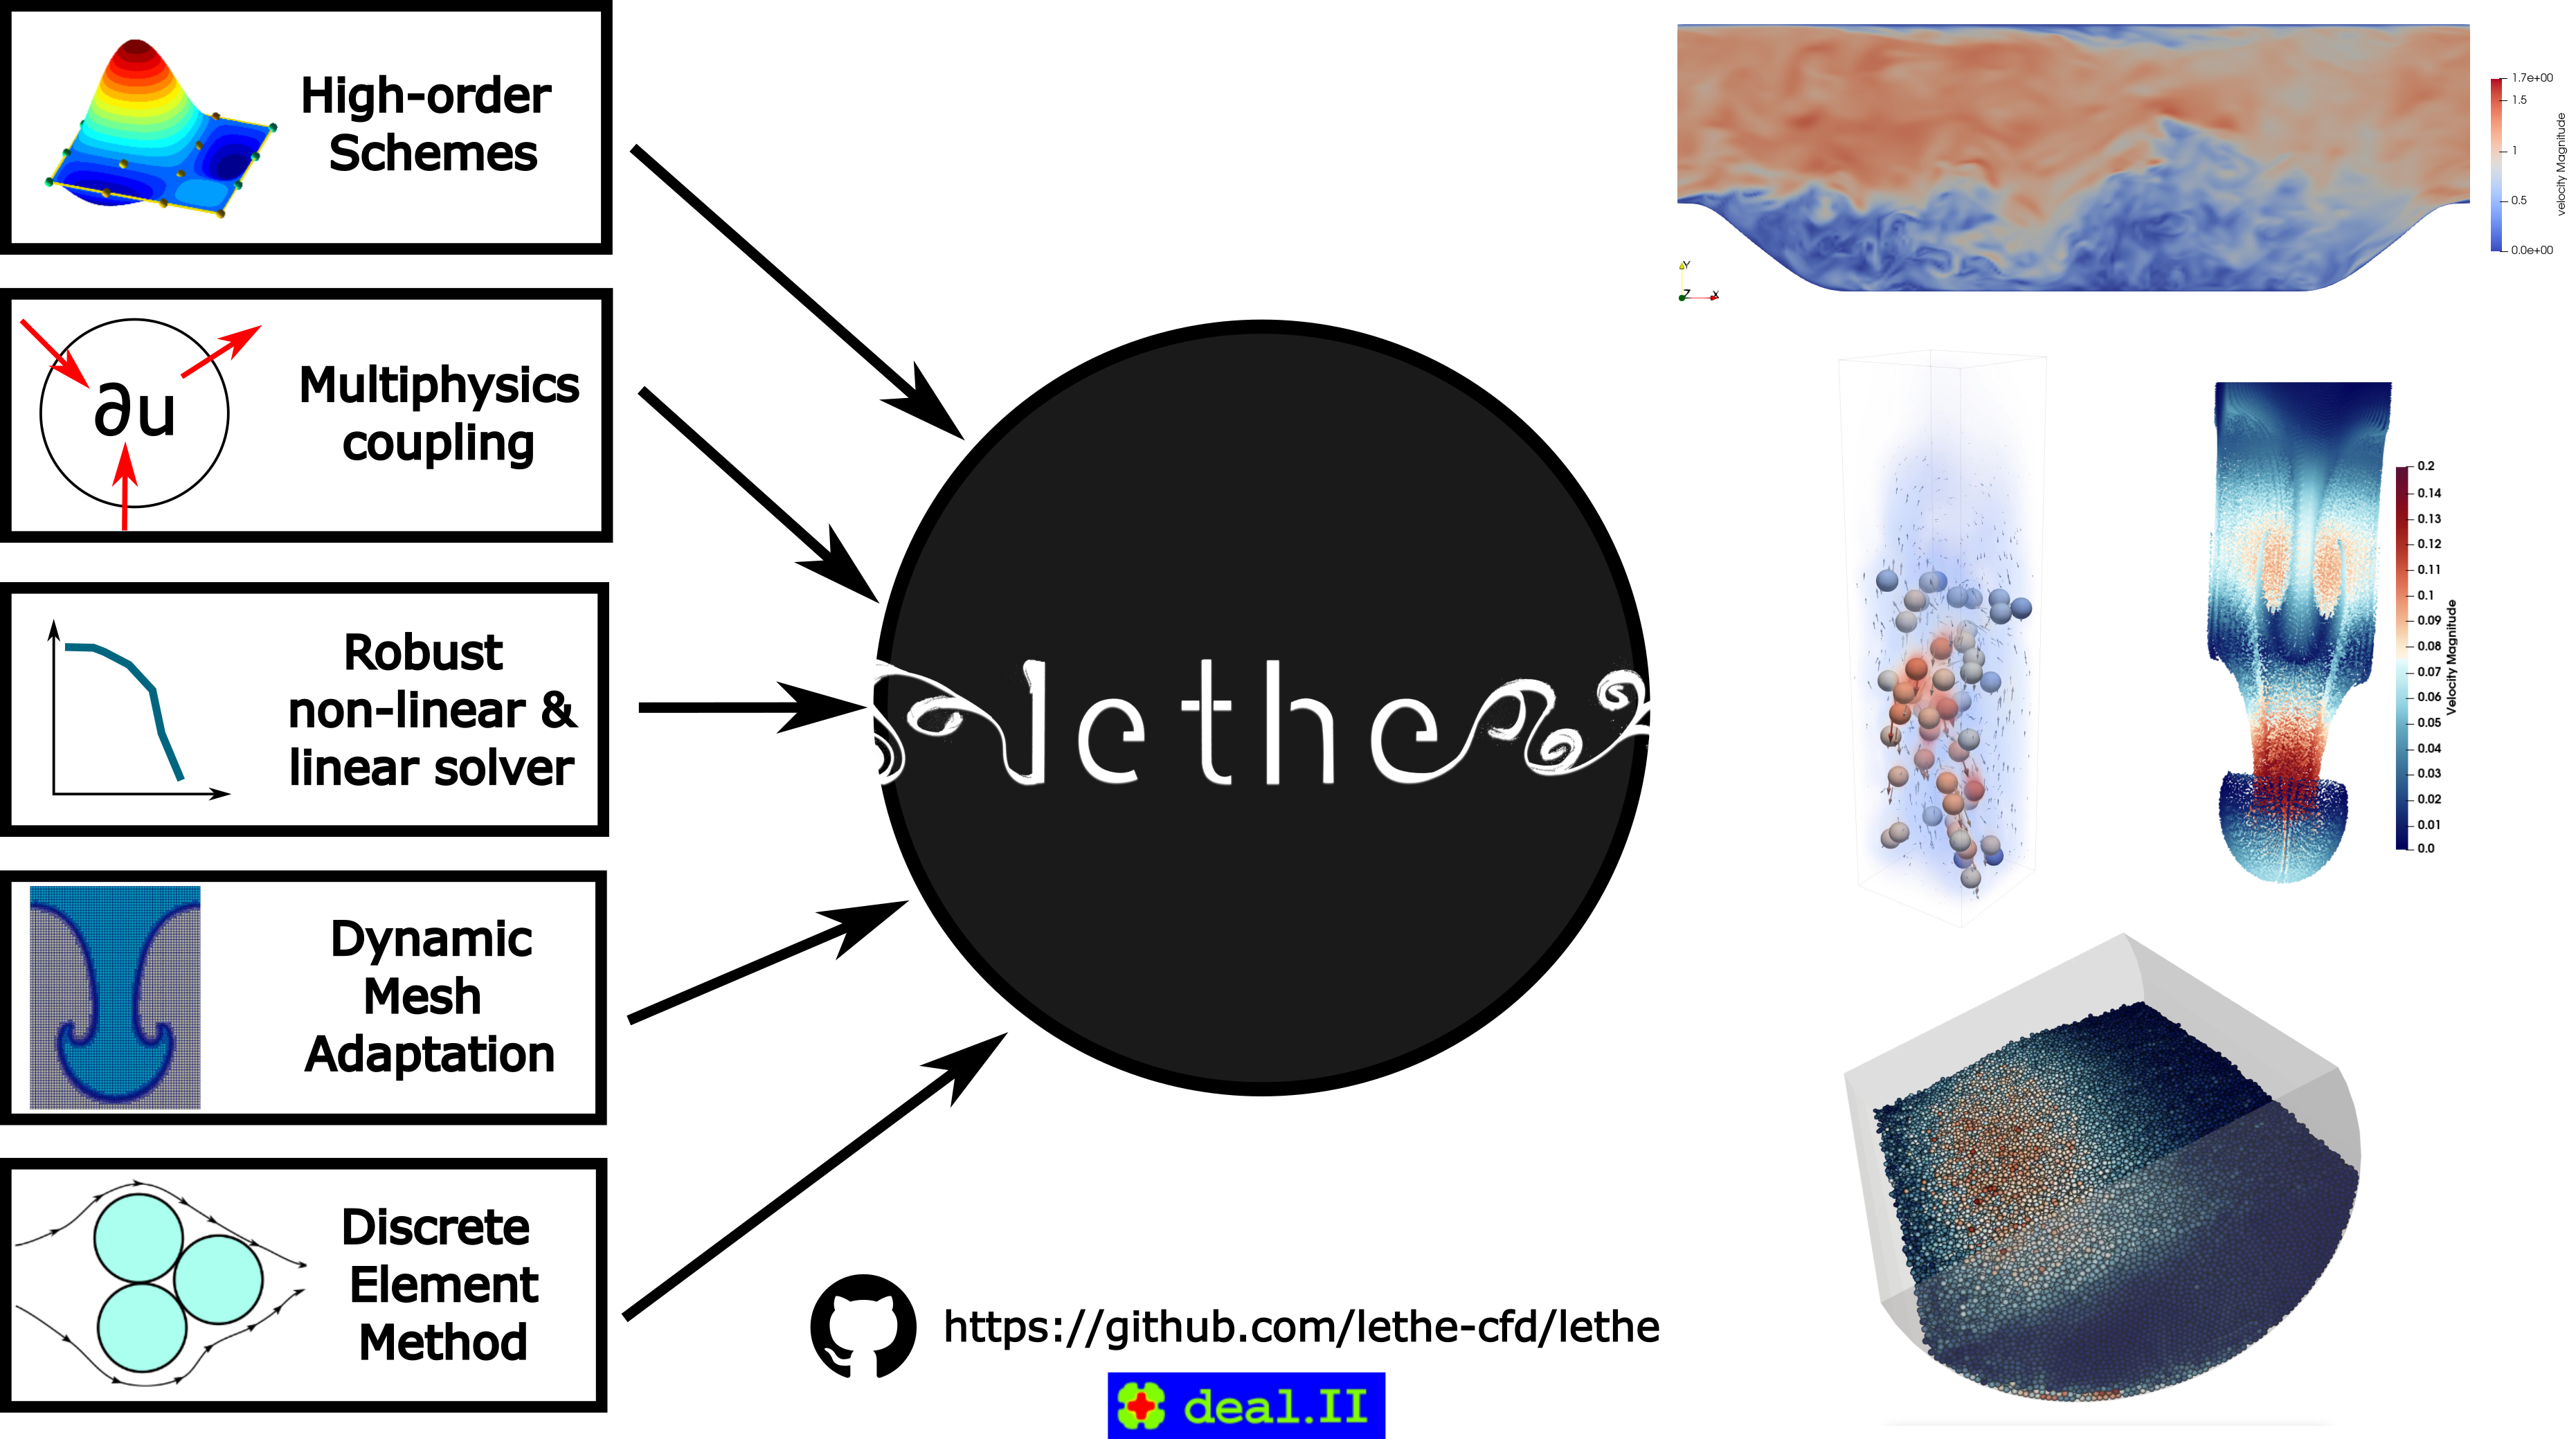
\includegraphics[width=0.94\paperwidth, height=0.94\paperheight]{images/splash.png}};
    \end{tikzpicture}	
 \end{frame}
	
\setbeamertemplate{footline}{} %this line removes slides numbers from references and additional slides
\begin{frame}[allowframebreaks, noframenumbering]
	\frametitle{\textbf{References}}
    \bibliographystyle{IEEEtran}
    \footnotesize
    \bibliography{references.bib}
\end{frame}    

% Additional slides
% This part is to add information that might be useful to answer questions
\begin{frame}[noframenumbering]
	\frametitle{\textbf{Additional slide:}}

\end{frame}
\end{document}